%% Copyright 2013 Kevin Ryde
%%
%% This file is part of Math-PlanePath.
%%
%% Math-PlanePath is free software; you can redistribute it and/or modify it
%% under the terms of the GNU General Public License as published by the Free
%% Software Foundation; either version 3, or (at your option) any later
%% version.
%%
%% Math-PlanePath is distributed in the hope that it will be useful, but
%% WITHOUT ANY WARRANTY; without even the implied warranty of MERCHANTABILITY
%% or FITNESS FOR A PARTICULAR PURPOSE.  See the GNU General Public License
%% for more details.
%%
%% You should have received a copy of the GNU General Public License along
%% with Math-PlanePath.  If not, see <http://www.gnu.org/licenses/>.


%% ----------------------------------------------------------------------------
%% plain tex

\input tikz.tex
\usetikzlibrary{lindenmayersystems}

\pgfdeclarelindenmayersystem{Dragon curve}{
  \symbol{S}{\pgflsystemdrawforward}
  \rule{F -> F+S}
  \rule{S -> F-S}
}
\tikzpicture
\draw
  [lindenmayer system={Dragon curve, step=10pt, axiom=F, order=8}]
  lindenmayer system;
\endtikzpicture
\bye



%% ----------------------------------------------------------------------------
%% angle 45 so direction across is fixed, using foreach

\documentclass{article}
\usepackage{tikz}
\usetikzlibrary{lindenmayersystems}
\begin{document}

\pgfdeclarelindenmayersystem{Dragon curve}{
  \symbol{S}{\pgflsystemdrawforward}
  \rule{F -> -F++S-}
  \rule{S -> +F--S+}
}

\foreach \x in {1,...,7} {
  \hbox{
    order=\x
    \hspace{.5em}
    \begin{tikzpicture}[baseline=0pt]
    \draw
      [lindenmayer system={Dragon curve, step=10pt,angle=45, axiom=F, order=\x}]
      lindenmayer system;
    \end{tikzpicture}
    \hspace{1em}
  }
  \vspace{.5ex}
}
\end{document}
\bye



%% ----------------------------------------------------------------------------
%% angle 45 so direction across is fixed

\documentclass{article}
\usepackage{tikz}
\usetikzlibrary{lindenmayersystems}
\begin{document}

\pgfdeclarelindenmayersystem{Dragon curve}{
  \symbol{R}{\pgflsystemdrawforward}
  \rule{F -> -F++R-}
  \rule{R -> +F--R+}
}

one
\begin{tikzpicture}[baseline=0pt]
\draw
  [lindenmayer system={Dragon curve, step=10pt,angle=45, axiom=F, order=1}]
  lindenmayer system;
\end{tikzpicture}
\hspace{1em}
two
\begin{tikzpicture}[baseline=0pt]
\draw
  [lindenmayer system={Dragon curve, step=10pt,angle=45, axiom=F, order=2}]
  lindenmayer system;
\end{tikzpicture}
\hspace{1em}
three
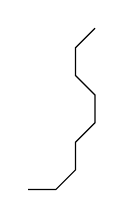
\begin{tikzpicture}[baseline=0pt]
\draw
  [lindenmayer system={Dragon curve, step=10pt,angle=45, axiom=F, order=3}]
  lindenmayer system;
\end{tikzpicture}
\hspace{1em}
four
\begin{tikzpicture}[baseline=0pt]
\draw
  [lindenmayer system={Dragon curve, step=10pt,angle=45, axiom=F, order=4}]
  lindenmayer system;
\end{tikzpicture}
\hspace{1em}
five
\begin{tikzpicture}[baseline=0pt]
\draw
  [lindenmayer system={Dragon curve, step=10pt,angle=45, axiom=F, order=5}]
  lindenmayer system;
\end{tikzpicture}

\vspace{5ex}
eight
\hspace{1em}
\begin{tikzpicture}[baseline=0pt]
\draw
  [lindenmayer system={Dragon curve, step=10pt,angle=45, axiom=F, order=8}]
  lindenmayer system;
\end{tikzpicture}

\end{document}
\bye


%% ----------------------------------------------------------------------------
%% latex

\documentclass{article}
\usepackage{tikz}
\usetikzlibrary{lindenmayersystems}
\begin{document}

\pgfdeclarelindenmayersystem{Dragon curve}{
  \symbol{R}{\pgflsystemdrawforward}
  \rule{F -> F+R+}
  \rule{R -> -F-R}
}
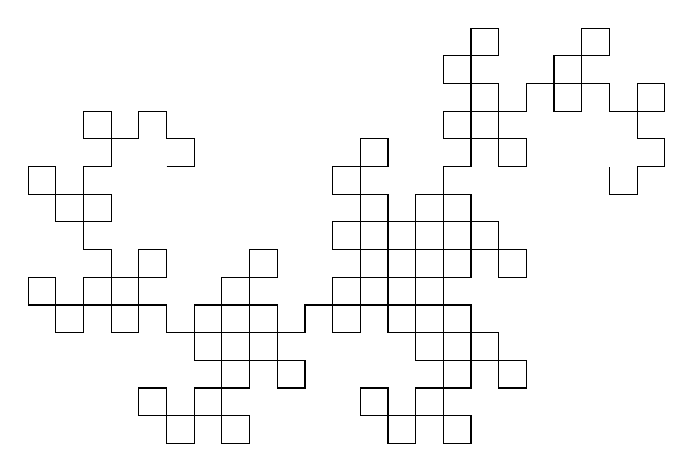
\begin{tikzpicture}[baseline=0pt]
\draw
  [lindenmayer system={Dragon curve, step=10pt, axiom=F, order=8}]
  lindenmayer system;
\end{tikzpicture}

\end{document}
\bye


%% ----------------------------------------------------------------------------
%% levels of expansion

\documentclass{article}
\usepackage{tikz}
\usetikzlibrary{lindenmayersystems}
\begin{document}

\pgfdeclarelindenmayersystem{Dragon curve}{
  \symbol{R}{\pgflsystemdrawforward}
  \rule{F -> F+R+}
  \rule{R -> -F-R}
}

one
\begin{tikzpicture}[baseline=0pt]
\draw
  [lindenmayer system={Dragon curve, step=10pt, axiom=F, order=1}]
  lindenmayer system;
\end{tikzpicture}
\hspace{1em}
two
\begin{tikzpicture}[baseline=0pt]
\draw
  [lindenmayer system={Dragon curve, step=10pt, axiom=F, order=2}]
  lindenmayer system;
\end{tikzpicture}
\hspace{1em}
three
\begin{tikzpicture}[baseline=0pt]
\draw
  [lindenmayer system={Dragon curve, step=10pt, axiom=F, order=3}]
  lindenmayer system;
\end{tikzpicture}
\hspace{1em}
four
\begin{tikzpicture}[baseline=0pt]
\draw
  [lindenmayer system={Dragon curve, step=10pt, axiom=F, order=4}]
  lindenmayer system;
\end{tikzpicture}
\hspace{1em}
five
\begin{tikzpicture}[baseline=0pt]
\draw
  [lindenmayer system={Dragon curve, step=10pt, axiom=F, order=5}]
  lindenmayer system;
\end{tikzpicture}
\hspace{1em}

\vspace{5ex}
eight
\hspace{1em}
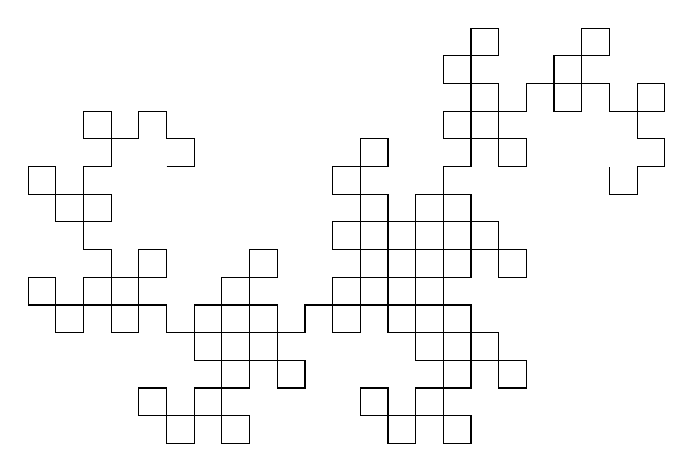
\begin{tikzpicture}[baseline=0pt]
\draw
  [lindenmayer system={Dragon curve, step=10pt, axiom=F, order=8}]
  lindenmayer system;
\end{tikzpicture}

\end{document}
\bye


%% ----------------------------------------------------------------------------

%% \begin{document}
%% \begin{tikzpicture}
%% \pgfdeclarelindenmayersystem{Dragon curve}{
%%   \symbol{R}{\pgflsystemdrawforward}
%%   \rule{F -> +F--R+}
%%   \rule{R -> -R++F-}
%% }
%% \draw
%%   [lindenmayer system={Dragon curve, step=10pt, angle=45,angle=45, axiom=F, order=3}]
%%   lindenmayer system;
%% \end{tikzpicture}
%% \end{document}
%% \bye

%% \begin{tikzpicture}
%% \draw [green!50!black, rotate=90]
%%   [l-system={rule set={L -> L+R+, R -> R-L-}, axiom=L, order=5, step=5pt, angle=90}]
%%   lindenmayer system;
%% \end{tikzpicture}
%% 
%% picture

%% \begin{tikzpicture}
%% \pgfdeclarelindenmayersystem{Dragon curve}{
%%   \rule{L -> L+RF+}
%%   \rule{R -> -FL-R}}
%% }
%% \draw
%%   [rotate=0]
%%   [l-system={Dragon curve, step=10pt, angle=90, axiom=FL, order=7}]
%%   lindenmayer system;
%% \end{tikzpicture}
%% 
%% picture
%% \end{document}
